\chapter{Experimental Methods}
이 장에서는 중성자 헤일로 핵의 구조상 특징에서 기인하는 soft E1 Excitation과 그것을 조사하는 방법인 Coulomb Dissociation에 대해 설명한다. 최종적으로, reduced transition probability B(E1)을 구하는 방법에 대해 설명한다.

\section{Soft E1 Excitation in Neutron Halo Nuclei}
왜 E1인지 설명
\section{Coulomb Dissociation}

\subsection{Invariant Mass Method}
납 타겟과 반응 직후 soft e1 excitation이 일어난 17b상태를 조사하기 위해서는 Invariant Mass Method로 상태를 재구성 할 필요가 있다. Excitation Energy는 다음과 같이 표시된다
\begin{displaymath}
{E}_{x}={S}_{2n}+{E}_{rel}
\end{displaymath}
여기서 ${S}_{2n}$은 중성자 분리 에너지, ${E}_{rel}$은 15B와 두 중성자 사이의 상대에너지이다. 
\subsection{Scattering Angle}

\section{Equivalent Photon Method}
우리는 납과의 전자기적 반응이 일어날 떄의 교환되는 가상 광자를 직접 검출 할 수 없다. 따라서 입사 빔의 에너지와 타겟과의 거리, 타겟의 종류
\begin{center}
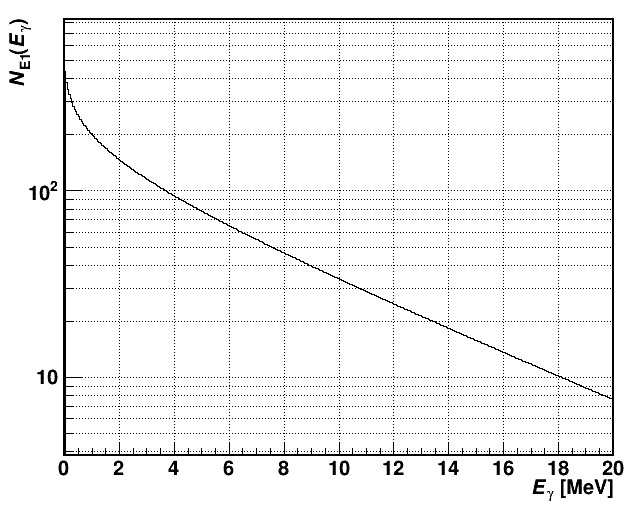
\includegraphics[width=8cm]{Figure/chapter2/virtual_photon_distribution.png}    
\end{center}
